\chapter{Aminas y compuestos nitrogenados}\label{ch:b2:amines}

El pescado que ya no está fresco huele a trimetilamina, una pequeña amina volátil.
Unas gotas de limón eliminan el olor: el ácido protona la amina, y
el ion amonio formado, al ser un ion, no puede evaporarse. El par no enlazante del nitrógeno
hace de las aminas bases y nucleófilos; unido a un carbonilo da \omterm{def:b2:amines:imine}{iminas},
a través de las cuales las proteínas llevan a cabo su química y los químicos fabrican aminas; y sobre
un anillo \omterm{def:b2:huckel:aromatic}{aromático} abre, mediante las sales de diazonio, el camino a los colorantes azoicos
que dieron color al siglo XIX.

\begin{recall}
El volumen del primer año: ácidos y bases de Brønsted, $\mathrm pK_a$ y diagramas de predominio,
nucleófilos y sustitución bimolecular, hemiacetales y acetales, dadores de hidruro,
organomagnesianos, clase de un carbono. \Cref{ch:b2:aromatic-substitution}:
nitración, reducción de los nitroarenos. El volumen escolar: aminas y amidas.
\end{recall}

\begin{omfigure}
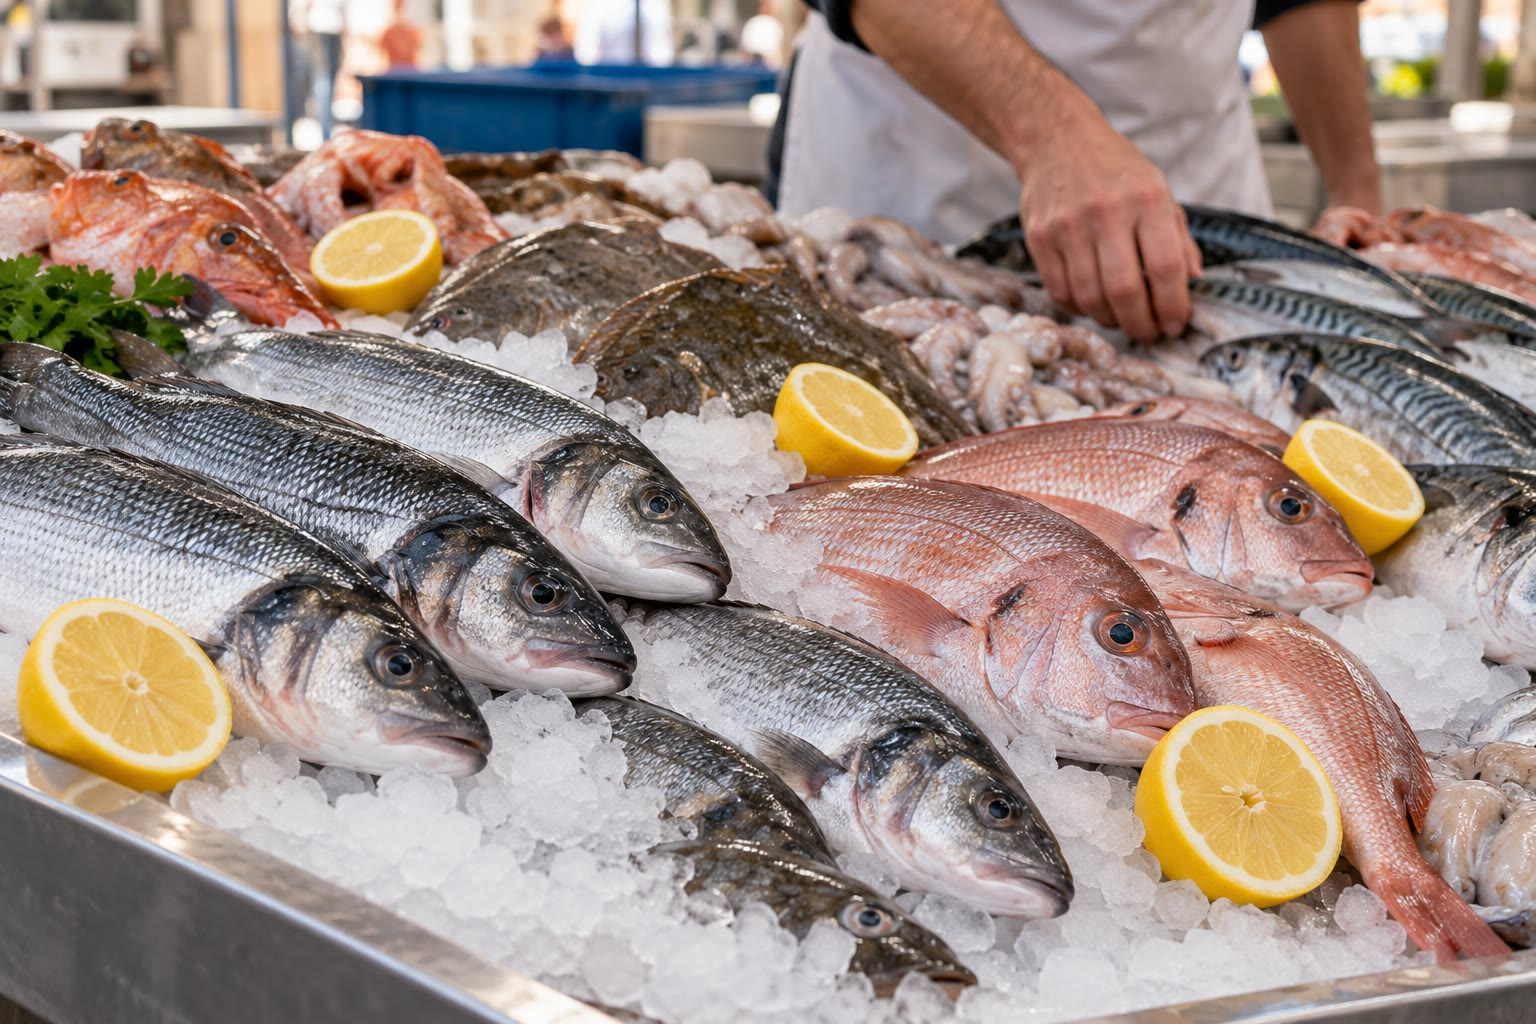
\includegraphics[width=0.6\linewidth]{images/book3/ai/b2-23-fish-stall.jpg}

{\small Un puesto de pescado: entre el pescado se colocan limones partidos por la mitad. Su ácido convierte la
trimetilamina del pescado en su ion amonio, no volátil.}
\end{omfigure}

\section{Estructura y basicidad}

\begin{definition}[Clases de aminas]\label{def:b2:amines:class}
Una amina es una \emph{amina primaria}\index{amina primaria} \ce{RNH2}, una \emph{amina secundaria}
\index{amina secundaria} \ce{R2NH} o una \emph{amina terciaria}\index{amina terciaria}
\ce{R3N} según el número de grupos carbonados unidos al nitrógeno. Un \emph{ion amonio
cuaternario}\index{ion amonio cuaternario} \ce{R4N+} tiene cuatro, y ningún par no enlazante.
\end{definition}

El nitrógeno de una amina es aproximadamente tetraédrico, y el par no enlazante ocupa la cuarta
posición. Una \omterm{def:b2:amines:class}{amina terciaria} con tres grupos distintos es quiral en principio, pero no puede
resolverse: la molécula se invierte pasando por una disposición plana, como un paraguas en el viento,
miles de millones de veces por segundo a temperatura ambiente.

\begin{proposition}[Basicidad]\label{prop:b2:amines:basicity}
En agua, las alquilaminas son bases más fuertes que el amoníaco ($\mathrm pK_a$ de sus iones amonio
cercano a 10 u 11, frente a 9.26), las arilaminas mucho más débiles (anilinio 4.60), y las amidas apenas
básicas (etanamida protonada, unos $-0.6$).
\end{proposition}

\begin{proof}[Argumento]
Los grupos alquilo ceden densidad electrónica al nitrógeno (efecto inductivo) y estabilizan la
carga positiva del ion amonio. En agua también cuenta la solvatación por enlaces de hidrógeno: un
ion con más enlaces \ce{N-H} está mejor solvatado, y por eso el trimetilamonio (9.80) es un
ácido más débil que el amonio, pero más fuerte que el dimetilamonio (10.73). En la anilina el par
no enlazante está deslocalizado en el anillo y se pierde al protonarse; en una amida está deslocalizado
sobre el oxígeno del carbonilo, y la protonación ocurre, débilmente, sobre el oxígeno.
% ledger: kb:NH3, pka:methylammonium, pka:dimethylammonium, pka:trimethylammonium, pka:anilinium, pka:ethanamideH
\end{proof}

\begin{omfigure}
\begin{tikzpicture}[font=\small, x=0.85cm]
  \draw[->, thick] (-1.5,0) -- (11.8,0) node[below right] {$\mathrm pK_a$};
  \foreach \x in {0,2,4,6,8,10} \draw (\x,0.1) -- (\x,-0.1) node[below, font=\scriptsize] {\x};
  \foreach \x/\l in {-0.6/{\ce{CH3CONH3+}}, 4.60/{\ce{C6H5NH3+}}} {
    \draw[omDef, thick] (\x,0) -- (\x,0.5);
    \node[font=\scriptsize, anchor=south] at (\x,0.5) {\l};
  }
  \foreach \x/\l/\y/\h in {9.26/{\ce{NH4+} (9.26)}/1.95/1.2, 9.80/{\ce{(CH3)3NH+} (9.80)}/1.45/0.85, 10.66/{\ce{CH3NH3+} (10.66)}/0.95/0.5, 10.73/{\ce{(CH3)2NH2+} (10.73)}/0.45/0.25} {
    \draw[omDef, thick] (\x,0) -- (\x,\h);
    \draw[black!40] (\x,\h) -- (12.2,\y);
    \node[font=\scriptsize, anchor=west] at (12.2,\y) {\l};
  }
  \node[font=\scriptsize, anchor=north west] at (-1.4,-0.5) {bases más débiles};
  \node[font=\scriptsize, anchor=north east] at (11.7,-0.5) {bases más fuertes};
\end{tikzpicture}

{\small $\mathrm pK_a$ de los ácidos conjugados de algunas bases nitrogenadas a
\qty{25}{\degreeCelsius}: cuanto más alto es, más fuerte es la base.}
% ledger: kb:NH3, pka:methylammonium, pka:dimethylammonium, pka:trimethylammonium, pka:anilinium, pka:ethanamideH
\end{omfigure}

\section{Las aminas como nucleófilos}

Las aminas atacan a los halogenoalcanos por sustitución bimolecular. El producto, una amina más
sustituida, es al menos tan nucleófilo como la de partida y compite por el halogenoalcano:
la alquilación del amoníaco da una mezcla de \omterm{def:b2:amines:class}{aminas primarias}, secundarias y terciarias y de la
sal cuaternaria.

\begin{proposition}[Polialquilación]\label{prop:b2:amines:polyalkylation}
La alquilación directa del amoníaco o de una \omterm{def:b2:amines:class}{amina primaria} da mezclas; solo la alquilación exhaustiva
hasta la sal de amonio cuaternario es limpia.
\end{proposition}

\begin{proof}[Argumento]
Cada alquilación deja un par no enlazante sobre un nitrógeno que el nuevo grupo alquilo hace más rico
en electrones; el producto reacciona con el halogenoalcano restante a una velocidad comparable. Solo cuando
al nitrógeno no le queda ningún par no enlazante, en \ce{R4N+}, se detiene la secuencia.
\end{proof}

Las \omterm{def:b2:amines:class}{aminas primarias} libres de sus parientes sobrealquilados se preparan de forma indirecta: por la vía de
Gabriel (alquilación del nitrógeno de la ftalimida, que lleva un único hidrógeno ácido, y luego
liberación de la amina), por reducción de un \omterm{def:b2:amines:nitrile}{nitrilo}, de una amida o de un compuesto nitro, o por
\omterm{def:b2:amines:reductive-amination}{aminación reductora} (véase más abajo).

\section{Iminas y enaminas}

\begin{definition}[Adición nucleófila]\label{def:b2:amines:nucleophilic-addition}
Una \emph{adición nucleófila}\index{adicion nucleofila@adición nucleófila} a un grupo carbonilo es el ataque de
un nucleófilo al carbono carbonílico, que pasa a ser tetraédrico, mientras el enlace $\pi$ \ce{C=O} se convierte en
un par no enlazante sobre el oxígeno.
\end{definition}

\begin{definition}[Hemiaminales, iminas y enaminas]\label{def:b2:amines:imine}
Una \omterm{def:b2:amines:class}{amina primaria} se adiciona a un aldehído o a una cetona dando un \emph{hemiaminal}\index{hemiaminal}
(un carbono que lleva \ce{OH} y \ce{NHR}); su deshidratación da una \emph{imina}\index{imina}
$\mathrm{R_2C{=}NR'}$. Una \omterm{def:b2:amines:class}{amina secundaria}, que no puede formar una imina neutra, da tras la deshidratación una
\emph{enamina}\index{enamina} $\mathrm{R_2C{=}CR{-}NR'_2}$, con el doble enlace desplazado al carbono contiguo.
\end{definition}

\begin{omfigure}
\setchemfig{atom sep=1.9em}
\schemestart
\chemfig{R_2C=O} \+ \chemfig{H_2N-R'}
\arrow{<=>}
\chemfig{R_2C(-[2]OH)-NH-R'}
\arrow{<=>[\ce{H+}][$-$ \ce{H2O}]}
\chemfig{R_2C=N-R'}
\schemestop
\par\vspace{6pt}

{\small Formación de una \omterm{def:b2:amines:imine}{imina}: la \omterm{def:b2:amines:nucleophilic-addition}{adición nucleófila} de la amina al carbonilo da el
\omterm{def:b2:amines:imine}{hemiaminal}; la catálisis ácida convierte su \ce{OH} en un grupo saliente (\ce{-OH2+}), sale el agua y
el par no enlazante del nitrógeno forma el doble enlace \ce{C=N}. Todas las etapas son reversibles: el agua en exceso
hidroliza de nuevo la \omterm{def:b2:amines:imine}{imina}.}
\end{omfigure}

\begin{proposition}[pH óptimo]\label{prop:b2:amines:imine-ph}
Las \omterm{def:b2:amines:imine}{iminas} se forman más deprisa en disolución ligeramente ácida, hacia pH 4 a 5.
\end{proposition}

\begin{proof}[Argumento]
La primera etapa necesita la amina libre (su par no enlazante); un medio demasiado ácido protona la amina
($\mathrm pK_a$ de unos 10) y elimina el nucleófilo. La deshidratación necesita ácido para protonar el
grupo hidroxilo; a pH alto es lenta. La velocidad, producto de ambas necesidades, es máxima en
un punto intermedio.
\end{proof}

\begin{definition}[Aminación reductora]\label{def:b2:amines:reductive-amination}
Una \emph{aminación reductora}\index{aminacion reductora@aminación reductora} convierte un compuesto carbonílico y una
amina en una amina más sustituida formando la \omterm{def:b2:amines:imine}{imina} (o el ion iminio) y reduciéndola en el
mismo recipiente, normalmente con cianoborohidruro de sodio \ce{NaBH3CN}.
\end{definition}

\begin{proposition}[Selectividad de la aminación reductora]\label{prop:b2:amines:reductive-amination}
A pH cercano a 6, el \ce{NaBH3CN} reduce el ion iminio mucho más deprisa que el compuesto carbonílico, de modo que
la amina se forma sin reducir el aldehído o la cetona a alcohol.
\end{proposition}

\begin{proof}[Argumento]
El grupo ciano hace del \ce{BH3CN-} un dador de hidruro débil, demasiado débil para un carbonilo neutro, pero
suficiente para un ion iminio protonado, cargado positivamente, un electrófilo mucho mejor.
\end{proof}

\section{Sales de diazonio}

\begin{definition}[Química del diazonio]\label{def:b2:amines:diazonium}
Un \emph{ion diazonio}\index{ion diazonio} es un catión \ce{R-N+#N}. La \emph{diazotación}\index{diazotacion@diazotación}
convierte una amina \omterm{def:b2:huckel:aromatic}{aromática} primaria en una sal de arildiazonio con nitrito de sodio y un ácido fuerte a
0--\qty{5}{\degreeCelsius}. En una \emph{reacción de Sandmeyer}\index{reaccion de Sandmeyer@reacción de Sandmeyer}, una sal de cobre(I)
(\ce{CuCl}, \ce{CuBr}, \ce{CuCN}) sustituye el grupo diazonio por Cl, Br o CN con pérdida de
dinitrógeno. En un \emph{acoplamiento azoico}\index{acoplamiento azoico}, el ion diazonio, un electrófilo débil,
ataca un anillo \omterm{def:b2:huckel:aromatic}{aromático} activado para dar un compuesto azoico $\mathrm{Ar{-}N{=}N{-}Ar'}$.
\end{definition}

\begin{proposition}[Estabilidad de los iones diazonio]\label{prop:b2:amines:diazonium}
Las sales de arildiazonio pueden conservarse en disolución acuosa fría y utilizarse; los iones alquildiazonio pierden
dinitrógeno de inmediato.
\end{proposition}

\begin{proof}[Argumento]
El dinitrógeno es un grupo saliente excelente (una molécula muy estable, una gran ganancia de entropía). Con un
grupo alquilo, la pérdida de \ce{N2} deja un carbocatión, o bien el agua lo ataca directamente: el ion no
sobrevive. Un catión arilo es muy inestable (un orbital $\sigma$ vacío en el plano del anillo,
no estabilizado por el sistema $\pi$), y el enlace \ce{C-N} del ion arildiazonio se
refuerza por conjugación con el anillo: a baja temperatura persiste; si se calienta, se descompone,
y el agua sustituye el grupo diazonio por \ce{OH}.
\end{proof}

\begin{omfigure}
\begin{tikzpicture}[font=\small, >={Stealth}]
  \node[cyclenode] (d) at (0,0) {\ce{Ar-N2+}};
  \foreach \a/\t/\c in {90/{\ce{Ar-Cl}}/{\ce{CuCl}}, 150/{\ce{Ar-Br}}/{\ce{CuBr}}, 210/{\ce{Ar-CN}}/{\ce{CuCN}},
                        270/{\ce{Ar-OH}}/{\ce{H2O}, caliente}, 330/{\ce{Ar-H}}/{\ce{H3PO2}}, 30/{$\mathrm{Ar{-}N{=}N{-}Ar'}$}/{\ce{ArH} activado}} {
    \node[cyclenode] (p\a) at (\a:2.6) {\t};
    \draw[->, thick] (d) -- (p\a) node[midway, font=\scriptsize, fill=white, inner sep=1pt] {\c};
  }
\end{tikzpicture}

{\small Reacciones de una sal de arildiazonio. El grupo \ce{N2+} se sustituye por un halógeno o por
cianuro (Sandmeyer, sales de cobre(I)), por \ce{OH} (agua caliente) o por H (ácido hipofosforoso), o
se conserva en un \omterm{def:b2:amines:diazonium}{acoplamiento azoico}.}
\end{omfigure}

\begin{method}[Vías a través de una sal de diazonio]\label{met:b2:amines:diazonium-routes}
\begin{enumerate}
  \item Úsese el grupo amino (un fuerte \omterm{def:b2:aromatic-substitution:directing}{orientador orto/para}) para colocar otros grupos, y conviértase después
        a través de la sal de diazonio.
  \item Sustitúyase por H para obtener disposiciones que la sustitución directa no puede dar
        (el 1,3,5-tribromobenceno a partir de la anilina).
  \item Sustitúyase por CN y luego hidrolícese a ácido carboxílico: una vía hacia un \ce{-COOH} sobre un anillo.
\end{enumerate}
\end{method}

\begin{method}[Preparar una amina]\label{met:b2:amines:make-amine}
\begin{enumerate}
  \item \omterm{def:b2:amines:class}{Amina primaria} sobre una cadena alquílica: vía de Gabriel, o reducción de un \omterm{def:b2:amines:nitrile}{nitrilo} (con un carbono
        más que el halogenoalcano usado para prepararlo) o de una amida.
  \item \omterm{def:b2:amines:class}{Amina secundaria} o terciaria: \omterm{def:b2:amines:reductive-amination}{aminación reductora} del compuesto carbonílico adecuado con
        la amina adecuada.
  \item Amina \omterm{def:b2:huckel:aromatic}{aromática}: nitración y luego reducción (hierro o estaño con ácido, o \omterm{def:b2:alkene-redox:hydrogenation}{hidrogenación
        catalítica}).
\end{enumerate}
\end{method}

\section{Nitrilos}

\begin{definition}[Nitrilo]\label{def:b2:amines:nitrile}
Un \emph{nitrilo}\index{nitrilo} es un compuesto \ce{R-C#N}, que se prepara por sustitución de un halogenoalcano
con cianuro o por una \omterm{def:b2:amines:diazonium}{reacción de Sandmeyer}.
\end{definition}

\begin{proposition}[Reacciones de los nitrilos]\label{prop:b2:amines:nitrile}
Un \omterm{def:b2:amines:nitrile}{nitrilo} se hidroliza, en medio ácido o básico, a la amida y luego al ácido carboxílico; el
hidruro de litio y aluminio lo reduce a la \omterm{def:b2:amines:class}{amina primaria} \ce{RCH2NH2}; un organomagnesiano
se adiciona a él una sola vez, y la hidrólisis de la \omterm{def:b2:amines:imine}{imina} formada da una cetona.
\end{proposition}

\begin{proof}[Argumento]
El carbono del \omterm{def:b2:amines:nitrile}{nitrilo} es electrófilo, como un carbono carbonílico: el agua (activada por un ácido, o en forma de
hidróxido) se adiciona a él, dando tras tautomería una amida, cuya hidrólisis se trata en el
\cref{ch:b2:acyl-substitution}. El hidruro se adiciona dos veces. Un organomagnesiano se adiciona una vez,
dando un anión \omterm{def:b2:amines:imine}{imina} que no sigue reaccionando; el agua hidroliza después la \omterm{def:b2:amines:imine}{imina} a la cetona.
\end{proof}

\begin{safety}{\ghs[5mm]{GHS03}\,\ghs[5mm]{GHS06}\,\ghs[5mm]{GHS08}\,\ghs[5mm]{GHS09}}
La anilina y la \textit{N},\textit{N}-dimetilanilina son tóxicas por contacto con la piel; el nitrito de sodio es
tóxico y oxidante; el cianoborohidruro de sodio desprende cianuro de hidrógeno en medio ácido y debe usarse
en una vitrina de gases. Las sales de diazonio secas pueden explotar: se mantienen siempre frías, en disolución, y se usan
de inmediato.
% ledger: ghs:aniline, ghs:dimethylaniline, ghs:NaNO2, ghs:NaBH3CN, ghs:sulfanilic-acid
\end{safety}

\section{Ejercicios}

\begin{exercise}[$\star$]\label{exo:b2:amines:1}
Dese la clase de: propan-1-amina, \textit{N}-metiletanamina, trietilamina,
cloruro de tetrametilamonio, anilina.
\end{exercise}

\begin{exercise}[$\star$]\label{exo:b2:amines:2}
Ordénense por basicidad creciente: amoníaco, metilamina, anilina, etanamida.
\end{exercise}

\begin{exercise}[$\star$]\label{exo:b2:amines:3}
Dense la \omterm{def:b2:amines:imine}{imina} formada a partir de la ciclohexanona y la metilamina, y las condiciones.
\end{exercise}

\begin{exercise}[$\star$]\label{exo:b2:amines:4}
A partir del cloruro de bencenodiazonio, dense los productos con \ce{CuBr}, con \ce{CuCN}, con agua caliente
y con fenol en medio básico.
\end{exercise}

\begin{exercise}[$\star\star$]\label{exo:b2:amines:5}
¿Qué forma de la trimetilamina predomina a pH 7, y en qué proporción? Explíquese el limón, y cómo puede
extraerse una amina de un disolvente orgánico hacia el agua.
\end{exercise}

\begin{exercise}[$\star\star$]\label{exo:b2:amines:6}
Dese la \omterm{def:b2:amines:imine}{enamina} formada a partir de la ciclohexanona y la pirrolidina, y explíquese por qué una \omterm{def:b2:amines:class}{amina secundaria}
no puede dar una \omterm{def:b2:amines:imine}{imina}.
\end{exercise}

\begin{exercise}[$\star\star$]\label{exo:b2:amines:7}
Prepárese la \textit{N}-bencilpropan-2-amina \ce{C6H5CH2NHCH(CH3)2} por \omterm{def:b2:amines:reductive-amination}{aminación reductora}: dense dos
pares de reactivos posibles.
\end{exercise}

\begin{exercise}[$\star\star$]\label{exo:b2:amines:8}
El benzonitrilo reacciona con bromuro de etilmagnesio y luego con ácido acuoso. Dese el producto.
\end{exercise}

\begin{exercise}[$\star\star$]\label{exo:b2:amines:9}
Escríbase la síntesis de Gabriel de la hexan-1-amina y explíquese por qué no da \omterm{def:b2:amines:class}{amina secundaria}.
\end{exercise}

\begin{exercise}[$\star\star\star$]\label{exo:b2:amines:10}
Prepárese el 1,3,5-tribromobenceno a partir de la anilina.
\end{exercise}

\begin{exercise}[$\star\star\star$]\label{exo:b2:amines:11}
Diséñese un colorante azoico a partir de la 4-nitroanilina y el fenol: escríbanse la \omterm{def:b2:amines:diazonium}{diazotación}, el acoplamiento (posición
y pH) y el producto.
\end{exercise}

\begin{exercise}[$\star\star\star$]\label{exo:b2:amines:12}
El hidróxido de amonio cuaternario de la \textit{N},\textit{N}-dimetilbutan-2-amina, calentado, da
principalmente but-1-eno. Explíquese esta orientación de Hofmann, opuesta a la regla de Zaitsev del volumen
del primer año.
\end{exercise}

\section{Problema: preparar el naranja de metilo}

\begin{problem}[{Problema de fin de semana --- el ácido sulfanílico y su \omterm{def:b2:amines:diazonium}{diazotación}, el \omterm{def:b2:amines:diazonium}{acoplamiento azoico} con la
\textit{N},\textit{N}-dimetilanilina, el naranja de metilo como indicador, y el rendimiento}]
\label{pb:b2:amines:1}
Datos: ácido sulfanílico (ácido 4-aminobencenosulfónico) \ce{C6H7NO3S}; naranja de metilo, la sal de sodio
\ce{C14H14N3NaO3S}; $\mathrm pK_a$ de la forma ácida del naranja de metilo 3.47. Masas molares
(\unit{g/mol}): C 12.011, H 1.008, N 14.007, O 15.999, Na 22.990, S 32.06. Operación (datos de ejercicio):
\qty{5.00}{g} de ácido sulfanílico, rendimiento del 80~\%.
% ledger: pka:methylorange, aw:C, aw:H, aw:N, aw:O, aw:Na, aw:S, ghs:sulfanilic-acid, ghs:NaNO2

\medskip
\noindent\textbf{Parte I --- El ácido sulfanílico y la \omterm{def:b2:amines:diazonium}{diazotación}.}
\begin{enumerate}
  \item El ácido sulfanílico existe como ion dipolar (zwitterión). Dibújese.
  \item ¿Por qué se disuelve primero en una disolución de carbonato de sodio?
  \item Escríbase la formación del ácido nitroso a partir del nitrito de sodio y el ácido clorhídrico.
  \item Escríbase la \omterm{def:b2:amines:diazonium}{diazotación} del ion 4-sulfonatoanilinio.
  \item ¿Por qué se lleva a cabo la reacción a 0--\qty{5}{\degreeCelsius}?
  \item ¿Qué cantidad de nitrito de sodio se necesita para \qty{5.00}{g} de ácido sulfanílico?
  \item ¿Por qué se comprueba la presencia de un ligero exceso de nitrito, y se destruye?
\end{enumerate}

\medskip
\noindent\textbf{Parte II --- El acoplamiento.}
\begin{enumerate}[resume]
  \item ¿Por qué la \textit{N},\textit{N}-dimetilanilina es un buen compañero?
  \item ¿En qué posición de su anillo ataca el \omterm{def:b2:amines:diazonium}{ion diazonio}, y por qué?
  \item Escríbase el producto (como sulfonato).
  \item ¿Por qué se lleva a cabo el acoplamiento en disolución débilmente ácida y no fuertemente ácida?
  \item ¿Por qué debe hacerse luego básica la disolución para precipitar la sal de sodio?
  \item ¿Por qué el \omterm{def:b2:amines:diazonium}{ion diazonio} es un electrófilo débil, que solo reacciona con anillos activados?
\end{enumerate}

\medskip
\noindent\textbf{Parte III --- Un indicador.}
\begin{enumerate}[resume]
  \item ¿De qué color es el naranja de metilo en medio básico, y en medio ácido?
  \item ¿Dónde capta un protón?
  \item ¿En qué intervalo de pH cambia de color?
  \item ¿Por qué el sistema conjugado extendido da un color visible?
  \item ¿Por qué la protonación desplaza la absorción?
\end{enumerate}

\medskip
\noindent\textbf{Parte IV --- Rendimiento.}
\begin{enumerate}[resume]
  \item Calcúlese la masa molar del ácido sulfanílico.
  \item Calcúlese la del naranja de metilo (sal de sodio).
  \item Calcúlese la cantidad de ácido sulfanílico utilizada.
  \item Calcúlese la masa teórica de naranja de metilo.
  \item ¿Qué pérdidas explican un rendimiento inferior al 100~\%?
  \item Indíquese la masa de naranja de metilo obtenida a partir de \qty{5.00}{g} de ácido sulfanílico con un rendimiento
        del 80~\%.
\end{enumerate}
\end{problem}
